\documentclass[10pt,a4paper,leqno]{article}
\usepackage{CJKutf8}
\usepackage[utf8]{inputenc}
\usepackage[T1]{fontenc}
\usepackage{amsmath,esint}
\usepackage{amsfonts}
\usepackage{amssymb}
\usepackage{xcolor}
\usepackage{mathrsfs}
\usepackage{makeidx}
\usepackage{graphicx}
\usepackage{float}
\usepackage{gensymb}
\usepackage{textcomp}
\usepackage{longtable}
\usepackage{ifpdf}
\usepackage{tikz}                            
\usetikzlibrary{shapes,arrows}               
%\usepackage{tgothic}
\ifpdf
\usepackage[breaklinks,hidelinks]{hyperref}
\else 
\usepackage{url}
\fi
\newcommand*\VF[1]{\mathbf{#1}}
\newcommand*\dif{\mathop{}\!\mathrm{d}}
\author{CBCO}
\title{eNotes: The Conic Section}
\date{}
\begin{document}
\maketitle

\noindent \numberwithin{equation}{section} % This line resets equation numbering when starting a new section. 
\renewcommand{\theequation}{\thesection.\arabic{equation}}  
%\renewcommand{\theequation}{Eq. \thesection.\arabic{equation}} % This line ads Eq.
 \par \ \par\noindent \numberwithin{figure}{section}
% \renewcommand{	heequation}{Eq. 	hesection.rabic{equation}}
 \par \ \par\noindent \begin{CJK*}{UTF8}{gbsn}
 \par \ \par\noindent \section{Introduction 介绍}
 \par \ \par\noindent A conic section is an intersection of a cone with a plnae.
 \par \ \par\noindent 圆锥曲线是圆锥体与平面的交线。
 \par \ \par\noindent In Figure 1.1, the cones were plotted with two different methods.
 \par \ \par\begin{figure}[H]
\centering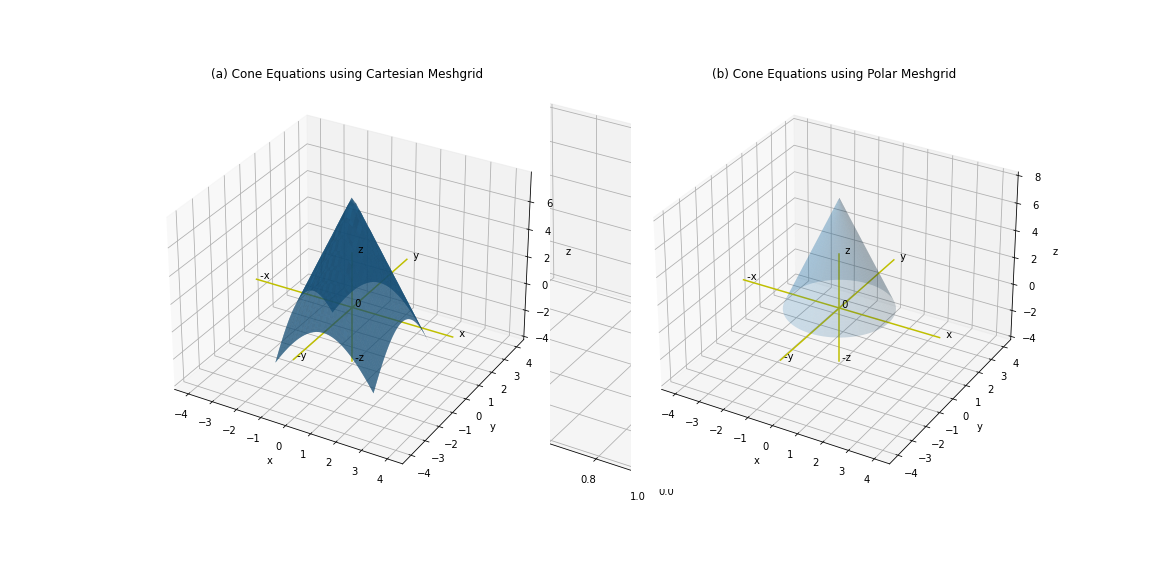
\includegraphics[width=1\linewidth,height=0.25\textheight]{Data/fgr01.png}
\caption{(a) Cone = f(x,y,z) plot (b) Cone = f(rho,phi,z) }
\label{fig:Data/fgr01.png}
\end{figure}

\noindent Open Cone01.py. Study the codes and run the file.
 \par \ \par\noindent The equation of cone can be found at \url{https://mathworld.wolfram.com/Cone.html} 
 \par \ \par\begin{equation}
 \begin{minipage}{250pt}
                \begin{flushleft} $\displaystyle x = \frac{b_{ase} \left(h_{eight} - u\right) \cos{\left(\phi \right)}}{h_{eight}}$  \end{flushleft}
 \end{minipage}
 \end{equation}
\begin{equation}
 \begin{minipage}{250pt}
                \begin{flushleft} $\displaystyle y = \frac{b_{ase} \left(h_{eight} - u\right) \sin{\left(\phi \right)}}{h_{eight}}$  \end{flushleft}
 \end{minipage}
 \end{equation}
\begin{equation}
 \begin{minipage}{250pt}
                \begin{flushleft} $\displaystyle z = u$  \end{flushleft}
 \end{minipage}
 \end{equation}
\begin{equation}
 \begin{minipage}{250pt}
                \begin{flushleft} $\displaystyle b_{ase} = 2$  \end{flushleft}
 \end{minipage}
 \end{equation}
\begin{equation}
 \begin{minipage}{250pt}
                \begin{flushleft} $\displaystyle h_{eight} = 8$  \end{flushleft}
 \end{minipage}
 \end{equation}
\begin{equation}
 \begin{minipage}{250pt}
                \begin{flushleft} $\displaystyle \operatorname{atan}{\left(\frac{h_{eight}}{b_{ase}} \right)} = 2 \operatorname{atan}{\left(\frac{r_{cone}}{h_{eight}} \right)}$  \end{flushleft}
 \end{minipage}
 \end{equation}
\begin{equation}
 \begin{minipage}{250pt}
                \begin{flushleft} $\displaystyle x^{2} + y^{2} = \frac{b_{ase}^{2} \left(h_{eight} - u\right)^{2}}{h_{eight}^{2}}$  \end{flushleft}
 \end{minipage}
 \end{equation}
\begin{equation}
 \begin{minipage}{250pt}
                \begin{flushleft} $\displaystyle x^{2} + y^{2} = \frac{\left(z - 8\right)^{2}}{16}$  \end{flushleft}
 \end{minipage}
 \end{equation}
\begin{equation}
 \begin{minipage}{250pt}
                \begin{flushleft} $\displaystyle \phi = \left[\begin{matrix}0\\0.0634665182543393\\\vdots\\6.28318530717959\end{matrix}\right]$  \end{flushleft}
 \end{minipage}
 \end{equation}
\begin{equation}
 \begin{minipage}{250pt}
                \begin{flushleft} $\displaystyle x = \left[\begin{matrix}2.0\\1.99597335294377\\\vdots\\2.0\end{matrix}\right]$  \end{flushleft}
 \end{minipage}
 \end{equation}
\begin{equation}
 \begin{minipage}{250pt}
                \begin{flushleft} $\displaystyle y = \left[\begin{matrix}0\\0.126847839313129\\\vdots\\-4.89858719658941 \cdot 10^{-16}\end{matrix}\right]$  \end{flushleft}
 \end{minipage}
 \end{equation}
\begin{equation}
 \begin{minipage}{250pt}
                \begin{flushleft} $\displaystyle z = 8 - 4 \sqrt{x^{2} + y^{2}}$  \end{flushleft}
 \end{minipage}
 \end{equation}
\noindent \section{Surface Plot of a Cone}
 \par \ \par\noindent The mathematical expression for surface plot is expressed as follows.
 \par \ \par\begin{equation}
 \begin{minipage}{250pt}
                \begin{flushleft} $\displaystyle z = f{\left(x,y \right)}$  \quad where x and y are independent variables\end{flushleft}
 \end{minipage}
 \end{equation}
\begin{equation}
 \begin{minipage}{250pt}
                \begin{flushleft} $\displaystyle x = f{\left(z,y \right)}$  \quad where z and y are independent variables\end{flushleft}
 \end{minipage}
 \end{equation}
\begin{equation}
 \begin{minipage}{250pt}
                \begin{flushleft} $\displaystyle y = f{\left(x,z \right)}$  \quad where x and z are independent variables\end{flushleft}
 \end{minipage}
 \end{equation}
\noindent The surface plots of a cone in Figure 1.1 were generated by cone01.py codes. The dependent variable is z and the independent variables are x and y. The equations of both plots are based on polar coordinate equations. The algorithms however are different.
 \par \ \par\noindent The surface plots requires a combination of two independent variables. The combination of two independent variables is produced by meshgrid function that has shape of a tuple of two values, that is for 100 values, the shape=(100,100). The independent variable must be expressed in terms of independent meshgrid independent variables. Hence, it must have the same shape of 2.
 \par \ \par\noindent \section{Intersection of a Cone and of a Plane}
 \par \ \par\noindent The equation of a plane is expressed as follows.
 \par \ \par\begin{equation}
 \begin{minipage}{250pt}
                \begin{flushleft} $\displaystyle A x + B y + C z + K = 0$  \end{flushleft}
 \end{minipage}
 \end{equation}
\begin{equation}
 \begin{minipage}{250pt}
                \begin{flushleft} $\displaystyle z = f{\left(x,y \right)} = - \frac{2 x}{5} + \frac{8 y}{5} + 5$  \end{flushleft}
 \end{minipage}
 \end{equation}
\noindent The equation above can create the plane as shown in Figure 3.1
 \par \ \par\begin{figure}[H]
\centering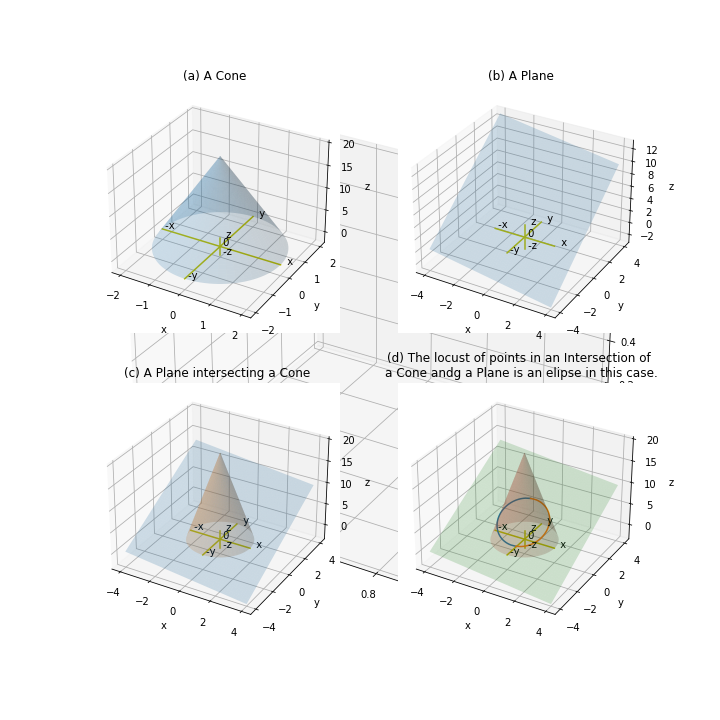
\includegraphics[width=1\linewidth,height=0.7\textheight]{Data/fgr02.png}
\caption{A plane overlapping with cone.}
\label{fig:Data/fgr02.png}
\end{figure}

\noindent The intersection of a cone and a plane defines a locus of points that can be expressed as equations of a line.
 \par \ \par\noindent The equations of a line consist of two equation of intersecting surfaces where two of the axes are dependent variable and the third axis is independent variable. The two equations for the surfaces can be solved for two variables and the third variable is the arbitrary variable or independent varialbe.
 \par \ \par\noindent \section{Conic Sections }
 \par \ \par\noindent The Figure 3 illustrate the mirrored cones that define conic section.
 \par \ \par\begin{figure}[H]
\centering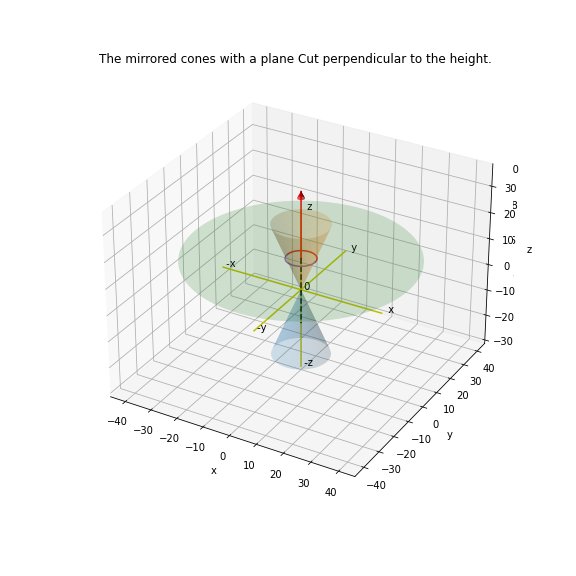
\includegraphics[width=1\linewidth,height=0.3\textheight]{Data/fgr03.png}
\caption{Cones that defined conic section.}
\label{fig:Data/fgr03.png}
\end{figure}

\noindent The disk plane intersecting with a cone generates a circle of locus of points.
 \par \ \par\begin{figure}[H]
\centering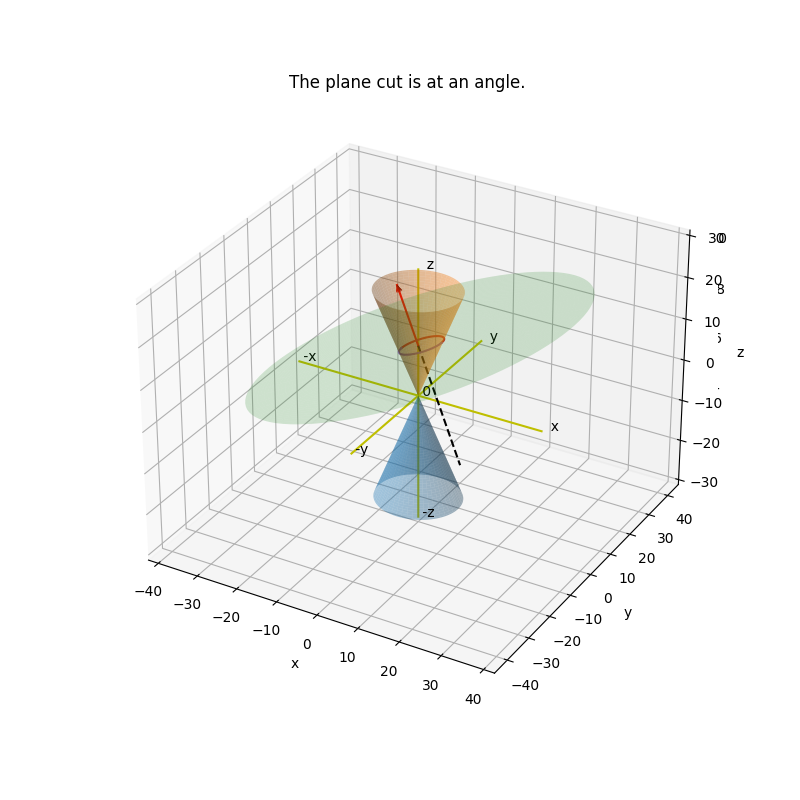
\includegraphics[width=1\linewidth,height=0.3\textheight]{Data/fgr04.png}
\caption{Cone cut by disk plane at an angle genrates an eliptical locus of points.}
\label{fig:Data/fgr04.png}
\end{figure}

\noindent \bibliographystyle{plain} 
 \bibliography{ccoLib/ccobib}
 \par \ \par\noindent \end{CJK*}
 \par \ \par\end{document}